%% This document gives an example on how to use the ntnubachelorthesis
%% LaTeX document class.
%% Use oneside for PDF delivery and twoside for printing in a book style
%% use language english, norsk, nynorsk and one of the following shortenings
%%  ``BSP'' Bachelor i Spillprogrammering,\\
%%  ``BRD'' Bachelor i drift av nettverk og datasystemer,\\
%%  ``BIS'' Bachelor i Informasjonssikkerhet,\\
%%  ``BPU'' Bachelor i Programvareutvikling, \\
%%  ``BIND'' Bachelor i Ingeniorfad - data, \\
%%  ``BADR'' Bachelor i drift av datasystemer, \\
%%  ``BIT'' Bachelor i informatikk, \\
%%  ``BABED'' Bachelor i IT-støttet bedriftsutvikling.
%%  ``BMS'' Bachelor i material science.
%%  ``BCE'' Bachelor i chemical science.  
%%   BPROG  Bachelor in Programming [Games|Applications]
%%   for example \documentclass[BCE,norsk,twoside]{ntnuthesis/ntnubachelorthesis}

\documentclass[BIND,english,oneside]{ntnuthesis/ntnubachelorthesis}

\usepackage{csvsimple}
\usepackage{booktabs}

\usepackage{gnuplottex}

\usepackage{svg}
\usepackage{imakeidx}
\usepackage{csquotes}
\usepackage{epigraph}
\usepackage{tabularx}
\usepackage{tikz}
\usetikzlibrary{graphs,graphdrawing,graphdrawing.trees}
\usepackage[super]{nth}

\definecolor{darkgreen}{rgb}{0,0.5,0}
\definecolor{darkred}{rgb}{0.5,0.0,0}

\lstset{ basicstyle=\ttfamily,
                keywordstyle=\color{blue}\ttfamily,
                stringstyle=\color{darkred}\ttfamily,
                commentstyle=\color{darkgreen}\ttfamily,
}


%Typesetting of C++
\newcommand{\CPP}[0]{{C\nolinebreak[4]\hspace{-.1em}\raisebox{.1ex}{\small\bf +\hspace{-.1em}+\ }}}



%\newcommand{\comment}[1]{\textcolor{blue}{\emph{#1}}}  %% use of the colour and you can see how to use commands with parts \comment{so what}

%% The class files defines these two
%% \newcommand{\NTNU}{Norwegian University for Science and Technology} %

% you can create you one #define like structures using the \newcommand feature
% you can change behaviour using \renewcommand

\newcommand{\com}[1]{{\color{red}#1}} % supervisor comment
%\renewcommand{\com}[1]{} %remove starting % to remove supervisor comments
% This will appear in text \com{Lecuters comment} and be visible unless you uncomment
% the renewcommand line.

\newcommand{\todo}[1]{{\color{green}#1}} % items to do
%\renewcommand{\todo}[1]{} %remove starting % to remove items to do

\newcommand{\n}[1]{{\color{blue}#1}} % other comment
%\renewcommand{\n}[1]{} %remove starting % to remove notes

\newcommand{\dn}[1]{} % add the d to a note to say that you have finished with it.

\newcommand{\gj}{NTNU i Trondheim}


% Norwegian Characters,  needs the {} or to be separate from the next letters
% \o{}   \aa{}   \ae{}   so at the end of a word you can use \o  \aa   \ae
% \O{}   \AA{}   \AE{}   you can also just leave a space and latex will remove it
%    eg, NTNU i Gj\o vik  or NTNU i Gj\o{}vik

\begin{document}

\thesistitle{Self-hosted Continuous Delivery and Deployment to Docker Swarm and Kubernetes}
\thesisshorttitle{Self-hosted continuous delivery and deployment to Docker Swarm and Kubernetes} % use this if you have a very long title and want something shorter on the header pages
\thesisauthor{Harald Floor Wilhelmsen}
\thesisauthorA{Erlend Tobiassen}
\thesisauthorB{Kenan Mahic}
\thesissupervisor{Jan Harald Nilsen}

% There use to be a number associated with projects, this would help identify which project was selected.  If you are told to add a project number then this line adds the number.
\oppgaveNo{065}

\nmtkeywords{Thesis, Bachelor, Continuous Deployment, Continuous Delivery, Self-hosting, Docker, Docker Swarm, Kubernetes, Security, Software, CI, CD}
\nmtdesc{The purpose of this project is to develop a Continuous Deployment and Delivery tool that can be hosted in local service-environments. Additionally, the purpose is to examine the security concerns surrounding tools for Continuous Deployment and Delivery running in cloud-based solutions compared to self-hosted tools. Many of the current tools are hosted externally, so using them requires exposing the service-environment’s API to the externally hosted solution. This is a security-risk the contractor wishes to avoid. With this goal in mind a design that circumvents these security risks was developed. Based on this design it is concluded that a self-hosted solution would avoid most security-risks involved in opening a management API.}

\nmtoppdragsgiver{\NTNU}
\nmtcontact{Runar Andersstuen, 90635272, \newline runar.andersstuen@trondheim.kommune.no}

\thesisdate{\ntnubachelorthesisdate}
\useyear{05.06.2018}

\nmtappnumber{} %number of appendixes
\nmtpagecount{} %currently auto calculated but might be wrong


\thesistitleNOR{Egen-hosted Tjeneste for Continuous Delivery og Deployment mot Docker Swarm og Kubernetes}
\nmtkeywordsNOR{Avhandling, Bachelor, Continuous Deployment, Continuous Delivery, Lokal, Docker, Docker Swarm, Kubernetes, Sikkerhet, Software, CI, CD}
\nmtdescNOR{Formålet med denne oppgaven er å utvikle et hjelpeverktøy for Continuous Deployment og Continuous Delivery som er mulig å kjøre i eget tjenestemiljø. Mulige sikkerhetshull blir undersøkt både i eget-hostede løsninger og eksterne løsninger. Mange nåværende løsninger for Continuous Delivery og Deployment baserer seg på skytjenester. I slike løsninger må tjenestemiljøene åpnes til styring fra internett, dette er en sikkerhetsrisiko som oppgavestiller ikke ønsket å ta. For å nå formålet ble det designet en løsning som unngår sikkerhetsrisikoene assosiert med styring fra internett. Basert på dette designet konkluderers det med at en løsning som kan kjøres på lokale tjenestemiljø eliminerer mange av sikkerhetsrisikoene tilhørende åpning mot internett.}
 % this is the file which contains all the details about your thesis

\makefrontpages % make the frontpages

% Dont indent paragraphs
\setlength{\parindent}{0em}
\setlength{\parskip}{8pt}

\chapter*{Preface} %the * means do not give the chapter a number
\label{chap:preface}

%Hvorfor ble oppgaven valgt? Skriv kort om prosessen som har ført fram til resultatet. 
%Husk å takke for hjelp og støtte fra ulike hold.
%Dato, sted, navn og underskrift av alle prosjektdeltakerne.
%Et forord i en rapport av denne typen bør ikke være på mer enn én side.
%Bacheloroppgave som videreføring av høstprosjekt: ”Arbeidsfordelingen” mellom de to emnene (fagene) beskrives her.
This bachelors assignment is written as the finalisation of our degree in computer science at NTNU. The motivation for this project from the group's point of view came from the desire to work with containerisation and new technologies. Since containerisation is one of the big new buzzwords this was a good opportunity to get acquainted with it. There is little focus on new technologies like this in the students' curriculum, so the participants of the project felt this was a good way to familiarise themselves with technology they will likely use in the future.


First of all we would like to thank our project supervisor Jan Harald Nilsen, for his help and advisory during our thesis. Secondly we would also like to extend thanks to Trondheim Municipality, especially Runar Andersstuen for their counsel and accommodations during the writing of the thesis. 

We would also like to thank Trondheim municipality's development team for their constant feedback and ideas.
% Elena for logo
The following assignment smtg stmg
% TODO smtg smtg


\tableofcontents
\listoffigures
\listoftables
\lstlistoflistings


\chapter{Introduction}
\label{chap:introduction}
\section{Motivation}
The TIP-team at Trondheim municipality had a desire for a more agile development process and wanted a continuous deployment setup for their applications. Though because of security concerns they decided that none of the solutions that were offered for- and compatible with their current environment were sensible to implement. This is where the idea for a self-hosted continuous deployment solution came from.

The need for the cion product came from security concerns raised by the TIP-team at Trondheim municipality. They have been users of Continuous Integration, and to some degree \acrfull{CD} for a while, but as the scope of their work grew, so did the need for added security and functionality. After careful review they came to the conclusion that the current solution of using bitbucket pipelines could not be expanded to supply \acrshort{CD} without introducing security risks. Bitbucket pipelines requires the user to expose a management API out to the open internet, which raises several security concerns that will be explored in detail in this document.

\section{Research and Hypothesis}
\begin{tabularx}{\linewidth}{X X}
    \epigraph{Developers and businesses avoid \acrshort{CD} out of fear for applications hosted outside their control.}{\textit{Research problem}}
    & \epigraph{Which, if any, security benefits arise from self-hosted \acrshort{CD} solutions, as opposed to cloud-based solutions?}{\textit{Research question}}
\end{tabularx}
As a result of using a self-hosted \acrshort{CD} solution the authors expect to see a reduced risk associated with use of \acrshort{CD}. It is possible that services that would be facing the internet in a cloud-based solution could be internal in a self-hosted solution. If so, each service available to the internet in all likelihood introduces multiple attack vectors to either the host or the user.

It is also speculated that some of the services facing the internet would need control of high risk infrastructure. A cloud-based \acrshort{CD} solution needs the ability to launch and restart applications running in critical environments, in the case of \acrshort{CD} even the production environment. If this is the case, trusting the cloud-solution, here a foreign entity, would pose a risk that any security aware user or group should be wary of. Even if the foreign entity is trustworthy they might be a competitor or otherwise unfit to have control over important infrastructure.

\section{Report Structure}
The report is structured into six main chapters that cover larger subjects. The chapters are further divided into multiple subsections. The six main chapters are the introduction, theory, technology \& method, results, discussion, and the conclusion \& future work

\textbf{Introduction} introduces the research question and explains the rest of the report.

\textbf{Theory} presents the theoretical background that we base our decisions and work on. 

\textbf{Technology and Method} explains the technologies used in the software project. 

\textbf{Scientific method} explains the methods used in the scientific research conducted in this project. 

\textbf{Results} presents the scientific, engineering and administrative results.

\textbf{Discussion} reflects on the results presented in the Results chapter. 

\textbf{Conclusion and Future Work} reflects on how much of the  original vision was actually achieved as well as presents features and changes that could be implemented in the future.

\section{Acronyms and Glossary}
Glossary and acronyms are listed in appendix \ref{glos} and additional technical terms \& explanations are described in the Terms and Definitions document.

% The purpose of this chapter is to lay a foundation for understanding the technical choices made in the following chapters.
\chapter{Theory}
\label{chap:theory}
\section{Database management system}

A database is a set of data held in computer storage, often structured for rapid retrieval and modification. A database management system is a system applications can interact with in order to retrieve and modify the data in databases.

As the web has reached a larger percent of the world's population it has grown. Both in numbers and in the professionalism expected by the average user. The number of requests large scale applications experience can in extreme cases reach millions of write operations per second\cite[p.~43]{nosql-ntnu}. Developer expectations of databases has altered to accommodate such use cases. 

\subsection{Distributed database}

Distribution is a paradigm for handling throughput larger than a single server can handle. Distributed databases consists of a network of physically separated computers and a system for maintaining the integrity of the database across multiple computers\cite[p.~4]{ddms}. This enables the database system to distribute the load over each machine, preferably to a computer physically near the client to ensure data localisation. Distributed databases have an advantage in performance and fault tolerance\cite[pp.~12--15]{ddms}.

\subsection{Document-oriented database}

Databases traditionally model relationships between data. These kinds of databases are called relational databases and a relational database management system (RDBMS) is used to enforce certain constraints on the data and the relationships between them. RDBMS are advantageous in ensuring well-formed data and validating queries. However there are problems with this approach for some use cases. NoSQL, of which document-oriented databases are a type, gives up on relational data and its advantages. However one can freely store data whose structure is not known in advance, as is commonly the case in big data. Like distributed databases it also comes with increased performance\cite{cmp-nosql} as there is simply less work for the database to do.

Document-oriented databases associate keys with structured data referred to as documents. The documents are usually stored in a standardised format like XML or JSON\cite[p.~9]{nosql-ntnu}. The document schemes are not constrained, and as such document-oriented databases fall under the NoSQL category.

\section{Continuous Integration}
As has been the truth for a while now, the world wants to become more agile. And as we have been delving deeper and deeper into this new world the need for new tools and methods to achieve this has increased. Continuous Integration was one of the first of these new additions, helping developers prevent integration problems, apply quality control and reduce delivery time. The main goal of CI was to detect and correct errors in the code base early, making them easier to handle. This is done through two key aspects. One is forcing developers to commit their changes daily, this makes the updates small and more manageable. The other key aspect is giving the developers swift feedback, this is done by running automatic tests on the build after committing changes. This new approach made it easier to work incrementally and by extension more agile. Most of the benefits of CI are just side effects, stemming from having to commit daily.

Most of these benefits are based on assumptions in the development world, and there are very few peer-reviewed articles either supporting or disproving these claims. This may be because the claims are hard to test, or there is little interest in the scientific community to answer these questions. Case studies from corporations though, seem to agree with a lot of these claims. But they should not necessarily be viewed as scientific, as they are not peer-reviewed. One of the few scientific articles on the subject though seems to suggest that CI does in fact increase the amount of releases. In fact it appeared that projects using CI had more than double the releases that projects without CI had. 

\begin{displayquote}
One of the more common claims about CI is that it helps
projects release more often, e.g., CloudBees motto is “Deliver
Software Faster” [6]. Over 50% of the respondents from our
survey claimed it was a reason why they use CI. We analyse
our data to see if we can indeed find evidence that would
support this claim.
We found that projects that use CI do indeed release more
often than either (1) the same projects before they used CI
or (2) the projects that do not use CI. In order to compare
across projects and periods, we calculated the release rate
as the number of releases per month. Projects that use CI
average .54 releases per month, while projects that do not
use CI average .24 releases per month. That is more than
double the release rate, and the difference is statistically
significant (Wilcoxon, p < 0.0000)\cite{hilton}.
\end{displayquote}

\section{Continuous Delivery}
Continuous Delivery came as an evolution on Continuous Integration. This new approach is based on making sure the build is deployment-ready at any given time. One would assume this makes the release process longer, as making sure your build is ready for production at any given time requires a bit more work than simply pushing your changes. The research however suggests this is not the case, in fact the following citation seems to suggest continuous deliver has numerous benefits,

\begin{figure}[h!]
  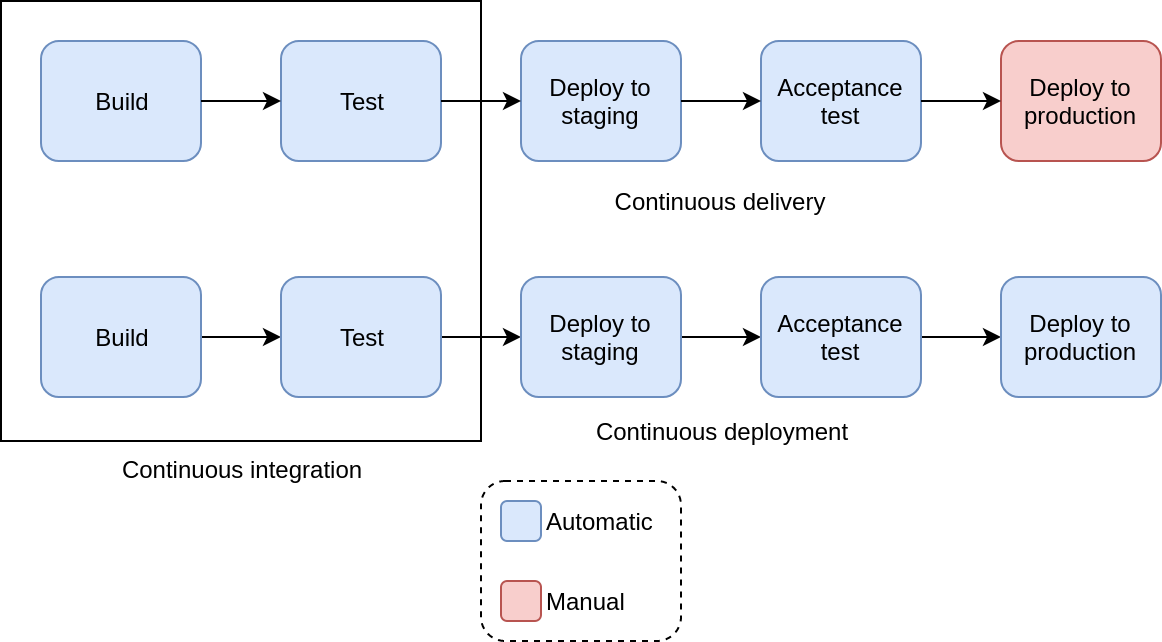
\includegraphics[width=\linewidth,height=\textheight,keepaspectratio]{images/ci_cd_comparison.png}
  \caption{CI/CD comparison}
  \label{fig:CI/CD-comparison}
\end{figure}

\begin{displayquote}
    The practices at the heart of continuous delivery help us achieve several important benefits:
    
    \textbullet ~Faster time to market. It’s not uncommon for the integration and test/fix phase of the traditional phased software delivery lifecycle to consume weeks or even months. When teams work together to automate the build and deployment, environment provisioning, and regression testing processes, developers can incorporate integration and regression testing into their daily work and completely remove these phases. We also avoid the large amounts of re-work that plague the phased approach\cite{continuousdeliveryfaster}.
\end{displayquote}

The advantages of continuous delivery benefit your corporation more than just in throughput and profitability. They increase employee satisfaction, which in and by itself increases worker productivity\cite{happy}.

\begin{displayquote}
    Firms with high-performing IT organisations were twice as likely to exceed their profitability, market share and productivity goals.
    High performers achieved higher levels of both throughput and stability.
    The use of continuous delivery practices including version control, continuous integration, and test automation predicts higher IT performance.
    Culture is measurable and predicts job satisfaction and organisational performance.
    Continuous Delivery measurably reduces both deployment pain and team burnout\cite{forsgren}.
\end{displayquote}

As cited, CD also has other advantages beneficial to organisations.

\section{Reactive programming}
Reactive programming is a paradigm applicable when continuous updates of information is preferred. Data that would traditionally be thought of as single data point is in reactive programming thought of as a stream of points over time. Streams can be transformed and combined to form new streams analogous to how cells in a spreadsheet depend on and update each other. Reactive programming enable elegant propagation of change throughout the domain it is applied to.

\newpage
\section{Security}
While \textit{attack vector} does not have a definition, in the nomenclature of computer security an attack vector usually refers to the path or mechanism by which a system is exploited or otherwise gained unauthorised access to\cite{av1}\cite{av2}\cite{av3}.


The sum of every possible attack vector constructs the \textit{attack surface} of a system. It follows that minimising the attack surface is desirable\cite[p.~1]{as} in a security context. The security community is working on quantitatively measuring the attack surface of a system. Intuitively one might measure the attack surface through the naive methods:

\begin{enumerate}
    \item Counting the number of bugs.
    \item Tracking known vulnerabilities.
\end{enumerate}

However Manadhata et al.\cite{as} suggest (1) is dependent on bug discovery. The process may miss---or have false positive---bugs, and it assigns equal severity to all bugs. (2) does not account for the system's configuration nor does the model capture future attackability.

Manadhata et al. define\cite{as} a method for measuring attack surface that they view as "meaningful and practical". By applying their method a set of attack classes common for CD tools can be built from the type hierarchy seen in figure \ref{fig:th}:

\begin{tabularx}{\textwidth}{| X | c |}
    \hline
    \textbf{Attack class}                  & \textbf{Payoff}\\ \hline \hline
    open\_TCP/UDP-socket                   & .3\\ \hline
    world-accessible\_TCP/UDP-socket       & .4\\ \hline
    open\_unsecured\_env-mgmt              & .6\\ \hline
    open\_secured\_env-mgmt                & .2\\ \hline
    world\_accessible\_secured\_env-mgmt   & .3\\ \hline
    third-party\_credentials               & 1\\ \hline
    world-accessible\_deployment-trigger   & .6\\ \hline
    locally-accessible\_deployment-trigger & .4\\ \hline
\end{tabularx}


\begin{figure}[h]
\makebox[\textwidth][c]{
\begin{tikzpicture}[]
  \begin{scope}
    [tree layout,level distance=10mm,text depth=.1em,text height=.8em, every node/.append style={font=\small}]
    \graph[fresh nodes] {
        all resources <- {
            channel <- {
                TCP or UDP socket <- {
                    world accessible,
                    open
                }
            },
            credentials <- third party trust,
            deployment trigger <- {
                locally accessible,
                world accessible
            },
            httpd module,
            environment management <- {
                unsecured <- {
                    open,
                },
                secured <- {
                    world accessible,
                    open,
                }
            }
        }
    };
  \end{scope}
\end{tikzpicture}
}
\caption{Type hierarchy of the properties in the CD domain}
\medskip
\small
\centering 
Leaf nodes represent attack classes.
\label{fig:th}
\end{figure}

\footnotetext{This figure is based on the type hierarchy example\cite{as} presented in the article by Manadhata et al.}

\textbf{httpd-module}: \begin{displayquote}
"This attack class consists of all resources of type \textit{httpd\_module}. CAN-2003-0789 describes a vulnerability  involving  handling  of  CGI  redirect  in  the \textit{mod\_cgid} module in \textit{apache} which an attacker can exploit to view sensitive information."\footnotemark[2]
\end{displayquote}

\textbf{open\_TCP/UDP-socket}: \begin{displayquote}
"The services  running  on  the system open TCP/UDP sockets and listen for client requests on them. Multiple sockets can be opened by a service and multiple services can share the same socket. This attack class is a subtype of the resource type channel. CVE-2001-0309 describes an attack involving open sockets since the \textit{inetd} daemon does not properly close sockets for internal services such as \textit{daytime} and \textit{echo}, an attacker can cause a denial-of-service attack by opening a series of connections to these services."\footnotemark[2]
\end{displayquote}

\footnotetext[2]{Quote taken from Manadhata et al.\cite{as}}

\textbf{world-accessible\_TCP/UDP-socket}: \begin{displayquote}
This attack class derives from the \textit{open\_TCP/UDP-socket} attack class, however it being accessible by anyone who knows the address increases the risk associated. It opens for the possibility of distributed denial-of-service attacks\cite{ddos}.
\end{displayquote}

\textbf{open\_unsecured\_env-mgmt}: \begin{displayquote}
An integral part of CD is the automatic deployment of programs to environments that run a class of programs. The environments needs to provide an API the CD solution can use to create and restart programs on certain triggers. This API provides attackers with free reign to manipulate programs in the environments if they get access to the network. 
\end{displayquote}

\textbf{open\_secured\_env-mgmt}: \begin{displayquote}
Like \textit{open\_unsecured\_env-mgmt} this class exposes an API for attackers, however the API is secured by TLS certificates, the CD is identified with a certificate signed by the environment. Certificates significantly reduce, but does not eliminate, the attackability of the API. RFC7457\cite{rfc7457} summarises known attacks, as such the possibility of future attacks is present.
\end{displayquote}

\textbf{world\_accessible\_secured\_env-mgmt}: \begin{displayquote}
This attack class is very similar to \textit{open\_secured\_env-mgmt}. Exposing a TLS protected management API to the world is not a big concern as TLS is in widespread use identifying owners of domains by website owners\cite{sslpulse}, and has proven itself not to be an easy target. However it does somewhat increase the associated risk compared to the \textit{open\_secured\_env-mgmt} class.
\end{displayquote}

\textbf{third-party\_credentials}: \begin{displayquote}
Since the CD solution requires access to the environment API an attacker could compromise the CD solution itself and gain access to the environment API through the CD tool. The certificate could also possibly be misused by the third party.
\end{displayquote}

\textbf{world-accessible\_deployment-trigger}: \begin{displayquote}
As part of a larger system CD solution often deploy based on external triggers. An attacker could fake such an external trigger, especially when some external triggers don't support any kind of identification\cite{docker-no-id}
\end{displayquote}

\textbf{locally-accessible\_deployment-trigger}: \begin{displayquote}
Like \textit{world-accessible\_deployment-trigger}, but does not allow external triggers.
\end{displayquote}
\chapter{Technology and Method}
\label{chap:process}

A lot of the technologies in use are the same that were used during the autumn project, with a few changes and additions. The particular technologies are outlined in subsections
\section{Technologies}

\subsection{Javascript + MithrilJS}
MithrilJS is a client side library for building single page web applications\cite{mithriljs}. It does well in performance-tests compared to AngularJS and React and the download-size is tiny in comparison\cite{mithril-framework-comparison}. It features a style of development that omits HTML, which is part of the reason as to why it was chosen.

\subsection{ReactiveJS}

\subsection{Python + AsyncIO}
AsyncIO is a module for python that provides infrastructure for single-threaded concurrent applications\cite{python-asyncio}. It is used in cion in the web API, backend and catalyst components. 

AIOHTTP is an asynchronous HTTP client and server for asyncio and python. In cion it is primarily used in the API-component for the web-page and the catalyst webhook component\cite{python-aiohttp}.

\subsection{RethinkDB}
RethinkDB is a JSON document store designed for real-time applications\cite{rethinkdb}. It was already in use before this project was started, and it was selected due to realtime communication being a central part of the cion solution and because cion does not really use relational data.

\subsection{Caddy}
Caddy, or caddyserver, is an easy-to-use web server with great support for HTTPS\cite{caddyserver}. It is used in cion on all components exposing a web-service. The reason it is used is to provide users with an easy way for cion to handle HTTPS on its own. Without caddy it would require the user to have some sort of a TLS termination proxy, though the user can still opt for the the latter solution if they want to do so.

\section{Distribution of Roles}
As is already noted in the project plan, the two main components of the project are the front- and backend. Harald Floor Wilhelmsen had the frontend as his main responsibility, while Erlend Tobiassen had the backend as his. Kenan Mahic had the role of researching how to extend cion to support Kubernetes, as well as making sure the front- and backend components worked well together. Even though people had their main responsibility, this did not mean we did not work each others parts. Everyone ended up having worked on every component. Both through providing help, and actually doing development 

\section{Scientific Method}
Evaluating security in a meaningful way has been a longstanding debate in the security community. There are few metrics, they are hard to measure, and it is difficult to actually ascertain anything from the few data points gathered. This makes it difficult to assess from both a quantitative and qualitative approach. For this paper though we have decided to go for a hybrid approach. As is mentioned in our theory, looking at the attack surface of theoretical self-hosted vs externally-hosted configurations will be the primary way in which the authors will conduct their quantitative research.

The authors applied their domain knowledge gained through developing a \acrshort{CD} solution to create a list of resources that potentially could be gained access to. From this list of resources the type hierarchy in figure \ref{fig:th} was developed. The list of attack classes was assigned an payoff based on how attractive, judged by the authors domain knowledge, of an target each attack class is. The attack surface measurement of each configuration was then calculated as the weighted sum $\sum n(S_i)\times w_i$ where $n(S_i)$ is the number of times attack class $i$ appeared in the configuration and $w_i$ is the payoff weight associated with attack class $i$. This gives us an measurement of the attack surface suitable for comparing the configurations against each other.

Qualitative results are created by interpreting the relative attack surfaces using deductive reasoning.
\chapter{Results}
\label{chap:results}

In this section we will present our results. The results in the scientific part will be in relation to our research question and hypothesis. In the engineering part we will present how many of product goals we achieved at time of delivery. Different types of tests also go under this part. The final part is where we will show all our administrative results. This includes project planning, time sheets and documentation of our development process.

\section{Scientific Results}
We will be comparing self-hosted solutions versus rival 

\begin{tabularx}{\linewidth}{|c||X|X|X|}
    \hline
    Deployment Tool & Hosted Externally & Third Party Access & Build-Trigger Exposed \\ \hline\hline
    Bitbucket Pipeline & YES & YES & YES \\ \hline
    Jenkins & NO\footnote{Unless Jenkins is hosted locally} & YES & YES \\ \hline
    Travis & YES & YES & YES \\ \hline
    Self-hosted & NO & NO & NO \\ \hline
\end{tabularx}

\section{Engineering Results}
% Planned features where implemented

% The feature implementation to add support for cion to deploy to Kubernetes turned out to be pretty simple compared to docker. This due to how Kubernetes requires
\subsection{Kubernetes support}
Kubernetes support was a highly regarded feature and was implemented as specified in the requirements document. Cion now has the ability to manage services in Kubernetes environments.


\subsection{Webhooks (Post-deploy behaviour)}
A new page that has been added to the web UI is the Webhooks page, it is used to configure the new webhook-feature. This feature allows the user to configure webhooks to trigger on specific events within the cion solution, for example when cion receives a new image or when a service is updated. 
Webhooks are highly configurable, thought this comes at the cost of them being complicated to configure, and does require a low-level understanding of the cion solution if the user wants to do something complicated. Though this is explained thoroughly in the end-user documentation. The complete list of configuration-options for webhooks is:

\begin{itemize}
    \item URL
    \item Headers
    \item Event
    \item Filters/triggers
    \item Body
\end{itemize}

The \textbf{URL} is the URL the webhook will send the \textit{POST}-request to.

The \textbf{headers} are what HTTP-headers to send to the URL.

The \textbf{event}-field is a select-box. The user has to select one, for example \textit{service-update}. 
When an event of the type selected occurs cion will run the events data through all the configured \textbf{filters}. The filters are regex-patterns that all have to match for the webhook to be fired. A filter is configured with a name and a value. The name is the name of the field in the event data, and the value is the regex-pattern that has to match that data for the filter to pass.

The \textbf{body} is the body of the HTTP-request to send to the configured URL. It supports the python format-function. So the user can insert fields from the event data into the body by using curly brackets around field-names in the text. For example:

\begin{verbatim}
    {{
        "service-name": "{service-name}"
    }}
\end{verbatim}

The above example generates a JSON-body containing exactly one key-value-pair, containing the service-name extracted from the event data. 
The user has to escape curly brackets, as shown above, due to how python's format-function tries to interpret them as variable-names.
The above body-string would result in something like the following when the field "service-name" in the event data is "cion\_api":

\begin{verbatim}
    {
        "service-name": "cion_api"
    }
\end{verbatim}

This example used JSON as the content type, but any string and formatting is supported. 

\subsection{Environments}
A new page was added where the user can configure and add environments for their cion instance to manage. It supports adding Kubernetes environments, and docker environments over TLS or the docker socket.


\subsection{Permissions}
A permissions system was implemented to allow administrators specify what features of cion a user should have access to. The admin can permit or deny access to service configuration on specific environments, environment configuration and cion-features like user-administration and log- and configuration-viewing.


\subsection{User settings/profile page}
The \textit{user settings}-, now named the \textit{profile}-page is implemented as specified in the requirements document. With fields to change the logged in user's password and gravatar-email. The user will only be able to change the password if they enter their old password. After changing their password they are logged out. 

\subsection{Service update scheduling (Scheduled deployment)}
The individual service page has gotten an upgrade and a new feature was added, service update scheduling. It allows users to schedule the updating of a service to a specific time and date.


\section{Administrative Results}
%Skriv om måloppfyllelse i forhold til framdriftsplan: Planen, slik den var tidlig i prosjektet, og virkeligheten. (Eventuelle kommentarer og forklaringer på at ting ble som de ble, skal skrives i neste kapittel.)

%Timeregnskap, samlet fordelt på timeforbruk og aktiviteter. Referer til kalendertid dersom det er relevant.

%Studenter med systemutviklingsprosjekt må dokumentere at utviklingsprosessen de har valgt virkelig er brukt, ved å beskrive hva som har skjedd når og til hvilke tidspunkter. Detaljene legges i vedlegg. For tyngre prosesser skal de enkelte trinnene framgå av timelister og statusrapporter. For smidige utviklingsprosesser må dere bruke fantasien når det gjelder å dokumentere: User stories, sprints, filmer, bilder av tavler er aktuelle muligheter.

\subsection{Goal Achievement}
%WORK IN PROGRESS
There were several deviations from our original project plan. Partly because we over-estimated some parts, and under-estimated others. We also did not consider the mandatory work in February in our first project plan, which meant we had to push some features down the line. The biggest deviations were for Kubernetes support and scheduled deployment. We severely underestimated the hours needed to integrate Kubernetes support, but this was partly balanced out by overestimating the hours needed to implement scheduled deployment. Kubernetes support was planned for finalisation by the end March, but ended up being finished in late April. Meanwhile scheduled delivery was due the middle of April but was already done at the start of March. The important dates chapter in the project plan contain the original planned due dates.
%HUSK OG ENDRE TIMEANSLAG OG GANT DIAGRAM PLZZZZZZ
%Discuss how we did compared to our project plan

\subsection{Process}
%Discuss how we went about development
Our development process was a mixture of several different agile methods with tweaks and adjustments. We used parts of SCRUM. We skipped daily stand-up meetings, but we did have weekly meetings with the product owner.  We used a SCRUM-board on Atlassian's Jira to manage and track tasks. We decided as a team to have core hours between 10.00-15.00 from Monday through Friday. Sprints was also a part of SCRUM we dropped. Even though we did not use sprints, we did work in an iterative manner. Every meeting with the product owner gave us more feedback that either changed or created tasks on our SCRUM-board.


\subsection{Documentation}
%Discuss how we documented, where it can be read and why we did it like we did.
Most of the documentation for cion is written in markdown\cite{github-markdown} formatting. This allows it to be hosted on sites like github.com and readthedocs.io. Hosting on github makes the documentation accessible for the target users for cion, which are developers and system administrators. Github is a development platform to host and review code and manage projects\cite{github}, most developers already have a relationship to it.

\chapter{Discussion}
\label{chap:discussion}

\section{Scientific}
%Hvorfor holdt hypotesene, eller hvorfor holdt ikke hypotesene? 
There is a quantifiable security advantage in using self-hosted CD solution. The authors saw that the security risk associated with using an self-hosted CD solution is significantly reduced as compared with using an externally hosted one. The risk assorted is dependant on, and grows with, the number of environments managed by the CD solution. In an external solution the risk per environment grows faster than in a self-hosted solution. A typical small scale team might have 3 environments---production, quality assurance and testing---in this case the attack surface of an external solution is 3.5 times as large as a self-hosted solution.

A large part of the attack surface consists of the services required for environment management and deployment triggers. In order for the services to work the environments and the CD solution needs to communicate with each other. This makes it impractical to avoid communication through the internet for externally hosted solution, this in turn exposes the services to a plethora of attackers that otherwise would have to get physical access.

In order for the CD solution to function it needs the ability to launch and restart applications running in the environments the solution is configured to manage. In the case of an externally hosted solution the certificates granting this permission has to be given out to the third party hosting the solution. This is a huge concern, even though these certificates can be revoked, as these certificates is often synonymous with admin access to the environment server.

%Drøft hvordan resultatene kan forstås i forhold til eller som svar på problemstillingen.
The research problem posed that "\textit{Developers and businesses avoid CD out of fear for applications hosted outside their control.}" Based on the results the authors are of the opinion that this fear is justified. As such there is a need for a CD solution that can be self-hosted and that is open-source so thatthe solutiont can be audited.

\subsection{Caveats}
\begin{itemize}
    \item The list of attack classes and their assigned payoff is not based on empirical fact but the authors knowledge of the systems and their implementation.
    \item The attack surface is measured of a minimal imagined CD solution, any specific implementation of a CD system, including the implementation by the authors, may have features that increase their attack surface.
    \item The results are only meaningful when compared with systems in terms of the same attack classes.
\end{itemize}

\section{Engineering}
% How did the end product turn out?
% Did the contractor get what they wanted?
% What requirements where fulfilled and what were not?
% Why did the results turn out as they did?
% What was good about how the features were implemented?
%    Write about how the webhooks feature opens up cion to be part of a larger chain of CI/CD. As in triggering other services to for example run integration tests after a deploy or similar.
% What was not so good?
All features the requirements in the requirements document where fulfilled. Some features and changes not specified in the requirements document were also implemented. These changes were namely a page in the web UI to add and configure environments, polishing of the UI on multiple pages, changes to existing features to make them easier to use and a log-view page that lets the user traverse and filter cion's deployment-logs.

A lot of the technologies used in the original fall project were new to the team members, which means that they learned a lot through the fall project. This resulted in some code written in unnecessarily complex or inefficient ways. A lot of cleanup was done through this project to make a lot of code cleaner and faster, and some elements in the UI was re-designed to create more consistency across the site. This makes the UI easier to use, because more of the pages now function in more similar ways.

All features except the listed "Post deploy behaviour" were directly requested by the contractor. The post-deploy feature was thought of by the team members and was implemented as "Webhooks". It was implemented because it allows cion to trigger other services after deployment. Which increases cion's applications.
An example of a setup where the webhooks-feature is very powerful would be as part of a larger CI/CD solution where staging-tests can be run automatically after an update has been deployed by cion. 
In such an example cion would deploy the newly built application to a staging-environment, which would trigger a webhook to be fired on a service to run integration tests on the application in the staging environment. The service running the tests would then send a webhook back to cion telling it to deploy the application to the production-environment.

\section{Administrative}
\epigraph{Give me five minutes to chop down a tree and I will spend the first two and a half sharpening my axe.}{Anonymous woodsman}
%Hva ble bra på grunn av valgt prosess, fremgangsmåte og teknologi?
The chosen hybrid project managements methodology allowed the team to work independently and to implement features the best way they saw fit, which resulted in a code base that the team was very comfortable with. This sets up the project for future work better than if a more strict project methodology was used. 

A semi-strict style-checking tool was introduced to encourage consistency across the code base. It did not strictly enforce a code style limiting the developers' creativity, but simply warned programmers when they wrote something that did not conform to the agreed upon style. Introducing this after a large chunk of the code base was already written, the fall-project that created the base software that this product is based upon, did lead to a lot of hours being spent on refactoring, but having a more consistent code base likely resulted in hours being saved as well, due to making the reading of each other's code easier. 

%Hva ble ikke bra på grunn av valgt prosess, fremgangsmåte og teknologi?

%Hva ble bra eller dårlig uavhengig av valgt prosess, fremgangsmåte og teknologi?


\subsubsection{Impact}
%Dere skal også drøfte arbeidet i forhold til et helhetlig systemperspektiv. Sett resultatene inn i en samfunnsmessig og økonomisk, eventuelt også miljømessig, sammenheng.

\subsubsection{Ethics}
%Analyser relevante etiskeproblemstillinger i forhold til resultatene fra arbeidet. Etikk-kompendiet fra 1.året kan være nyttig, se [Søraker 2013].
% TODO: We've made a self-hosted CD-solution. And this document concludes that self-hosted CD-tools are more secure than externally hosted / cloud-based solutions.
There are some ethical concerns regarding the relationship between the product developed as part of this assignment and this report. As part of the assignment the team has made an open-source self-hosted CI/CD-solution called cion, and are to research the security benefits in self-hosted solutions versus externally hosted solutions. The findings of the scientific part of this report conclude that self-hosted \acrshort{CD}-tools are more secure than externally hosted or cloud-based solutions. This could be viewed as self-promotion, so this part of the report is to inform the reader of the ethical concerns regarding a possible vested interest in regards to the conclusion.


\subsection{Group Dynamic}
The teamwork has mostly been free of problems. By dividing the work into distinct parts of responsibility you end up depending on each individual delivering on their end. This way of working works really well when it goes well, but can also end really bad. In case of one individual not delivering you have no one else to pick up the slack. This is partly mitigated by the fact that you tend to want to perform when you are relied on, and not be the one that is dragging the others behind. The alternative would be spreading the work across the entire group and working on the same parts together, some form of pairwise programming. This would lessen the problem of one team member slacking, and give fewer code defects. It would also be slower though, and need more man-hours for the same amount of work than if we were to work individually. This is the primary reason we chose to work independently, we weighed man-hours more important than the risks associated by working alone. Since everyone in the group was familiar with each other from previous projects, the risk of someone slacking was not concern at all.

Some parts did not work that well. Since this is a continuation of a previous project by a group with one new addition, the gap in knowledge between the new addition and the existing group can be substantial. So without a proper introduction or learning period, this can make it really hard for the new person to work independently and take initiative. If we were to do this over again we would definitely take some time at the start of the project to get the new person better acquainted with the system. This problem did get better over time though, but the situation would have bettered more quickly by investing more time in teaching the new member from the start. We would recommend anyone adding a new member to the continuation of a project to dedicate some time to familiarise the new person with the project. We would also recommend the group work together in the same room, the main reasons being it makes it easier to help each other and brainstorm ideas. As well as making it easier for the new member to ask for help when needed.

% Forslag til andre grupper som skal legge til et nytt team-medlem i overføring fra hostprosjekt til bachelor

\chapter{Conclusion and Future Work}
\label{chap:conclusion}
There is a security risk associated with using cloud based solutions for continuous delivery. These risks are alleviated by self-hosting a system. The security benefits from self-hosting originate from minimising the attack surface. Minimising the attack surface is accomplished by reducing the number of internet-facing services like containerisation environment management APIs and deployment triggers.

Although analysing the security of software systems can be challenging, the authors recommend the article \textit{"Measuring a System’s Attack Surface"} by Pratyusa Manadhata and Jeannette M. Wing as a starting point for quantitatively evaluating the attack surface of such systems.  

To alleviate some challenges with adding a new team member as discussed in \nameref{subsec:groupdynam}, the team would in retrospect have taken more time at the start of the project to get the new addition better acquainted with the system. This problem did get better over time, but the situation would have improved faster by investing more time in teaching the new member from the start. Another lesson learned would be that the group should work together in the same room; the main reason being it makes it easier to help each other and brainstorm ideas. 


% future work discuss and theory-craft if cion can be a build service as well, so cion would be a complete CI/CD-solution.
\section{Future Work}
The authors would like to see cion support building application images, like docker images, so that it could stand alone as a complete \acrshort{CI/CD} solution. This would allow for cion to be completely isolated behind a private network. This setup would require a locally hosted docker registry reachable from the same network that cion is running in. This would be possible due to cion no longer needing to be activated by an external source like Docker Hub or Bitbucket pipelines.

Another feature planned is further integration between cion and the environments it is managing. When cion already has access to management \acrshort{API}s, cion could extract real-time data on what applications are running where and application statuses \& states. This integration could also be extended to allow the managing of running applications through the cion web UI, like the ability to start, stop and deploy applications. Cion would then be an all-in-one solution supplying \acrlong{CI}, \acrlong{CD}, and application management.


\bibliographystyle{ntnuthesis/ntnubachelorthesis}
\bibliography{inc/BachelorExample}

\appendix %after this line all chapters will have letters instead of numbers
%\input{inc/projectplan}
%\input{inc/gantt}
%\input{inc/worklog}

\end{document}
